\subsection{Test 1:}

The first test consists to prove that the {\bfseries Hamiltonian-Cycle} in Figure 4.1.0 is actually one ( {\itshape C = [ 8, 9, 10, 11, 12, 13, 14, 15, 16, 17, 18, 19, 20, 1, 2, 3, 4, 5, 6, 7, 8 ]} ), so first we declare the graph in our program, for this we use something that python call {\itshape dictionary} which it's very similar to a {\itshape Hash-map}. The left elements of the ':' will be the nodes and right element is a list whit its adjacent vertices. We can corroborate this in Figure 4.1.0. After running the program we will have a console output ( Figure 4.1.1 ) and the plot of the computational time of the algorithm ( Figure 4.1.2 ). Finally the table 1 describe the point of Figure 4.1.2. \hfill \break

\begin{figure}[H]
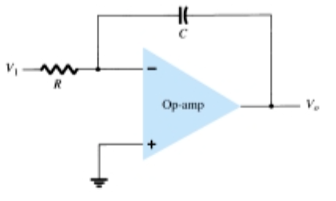
\includegraphics[height = 6cm, width = 8cm]{10.png}
\centering \linebreak \linebreak {\small Figure 4.1.0: Graph to analyze.}
\end{figure} \hfill \break

\begin{lstlisting}
def main ( ):
    graph = {
        1: [ 20, 2, 5 ],  2: [ 1, 18, 3 ], 3: [ 2, 16, 4 ], 4: [ 3, 5, 14 ],
        5: [ 4, 6, 1 ], 6: [ 5, 13, 7 ], 7: [ 8, 6, 20 ], 8: [ 7, 9, 12 ],
        9: [ 8, 19, 10 ], 10: [ 9, 17, 11 ], 11: [ 10, 15, 12 ], 12: [ 8, 13, 11 ],
        13: [ 12, 6, 14 ], 14: [ 13, 4, 15 ], 15: [ 14, 11, 16 ], 16: [ 15, 17, 3 ],
        17: [ 10, 16, 18 ], 18: [ 17, 2, 19 ], 19: [ 9, 18, 20 ], 20: [ 1, 19, 7 ]
    }
    certificate = [ 8, 9, 10, 11, 12, 13, 14, 15, 16, 17,
    	            18, 19, 20, 1, 2, 3, 4, 5, 6, 7, 8 ]
    verify_hamiltonian ( graph, certificate )
\end{lstlisting} \hfill \break

\begin{figure}[H]
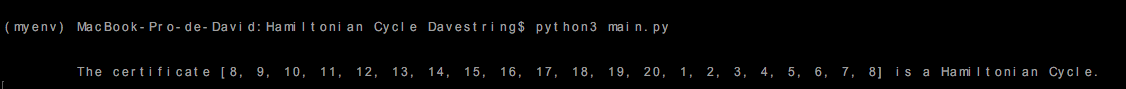
\includegraphics[height = 1.5cm, width = 16.5cm]{10c.png}
\centering \linebreak \linebreak {\small Figure 4.1.1: Console output.}
\end{figure} \hfill \break

\begin{figure}[H]
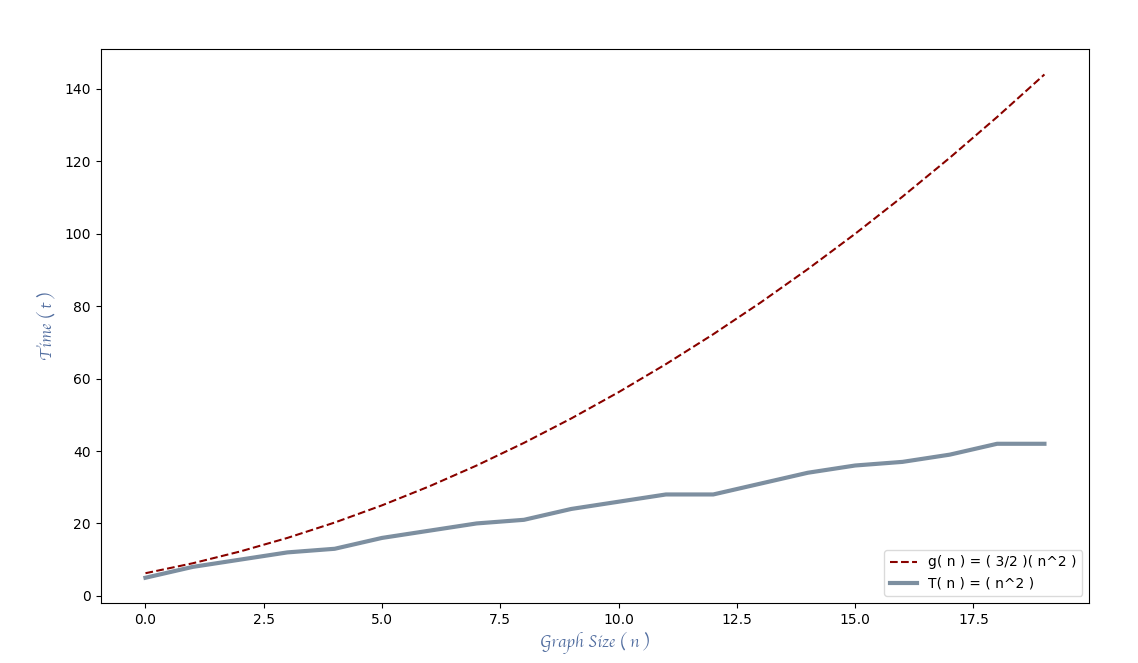
\includegraphics[height = 8cm, width = 16.5cm]{10g.png}
\centering \linebreak \linebreak {\small Figure 4.1.2: Plot of the algorithm.}
\end{figure} \hfill \break

{\bfseries\itshape\color{carmine}{Observation:}} {\itshape\color{carmine}{Figure 4.1.2 has 2 plots, the red one it's and asymptotic function $n^{2}$ for the blue one, which it's the computational time of the algorithm.}} \hfill \break

\begin{center}
\begin{tabular}{c c}
\toprule \toprule
\hspace{100px} Graph Size \hspace{90px} & \hspace{100px} Time \hspace{90px} \\
\midrule \midrule
0 & 5 \\
\midrule
1 & 8 \\
\midrule
2 & 10 \\
\midrule
3 & 12 \\
\midrule
4 & 13 \\
\midrule
5 & 16 \\
\midrule
6 & 18 \\
\midrule
7 & 20 \\
\midrule
8 & 21 \\
\midrule
9 & 24 \\
\midrule
10 & 26 \\
\midrule
11 & 28 \\
\midrule
12 & 28 \\
\midrule
13 & 31 \\
\midrule
14 & 34 \\
\midrule
15 & 36 \\
\midrule
16 & 37 \\
\midrule
17 & 39 \\
\midrule
18 & 42 \\
\midrule
19 & 42 \\
\bottomrule
\end{tabular}
\centering \linebreak \linebreak Table 1.
\end{center}

